\chapter{Metodologi}\label{c3}

\section{Pengenalan}
Metodologi pembangunan antaramuka pengguna bergrafik untuk mengautomasikan konfigurasi bagi sistem terbenam Linux yang juga dipanggil ELWI iaitu singkatan kepada \textit{"Embedded Linux Web Interface"} ini ialah satu set panduan lengkap yang mengandungi model-model, kemudahan peralatan (tool) dan teknik-teknik khusus yang perlu diikuti bagi melaksanakan setiap aktiviti yang terdapat dalam kitar hayat mereka dalam bidang ini. Metodologi yang didokumenkan ini boleh menjadi bahan rujukan kepada organisasi yang berkaitan bagi memahami pembangunan sesebuah sistem. 

Metodologi ini juga merupakan maklumat bertulis dalam bentuk buku atau dokumen bertulis mengandungi maklumat terperinci bagi setiap aktiviti yang perlu dilaksanakan oleh pembangunan sistem termasuk bentuk dokumentasi dan laporan-laporan yang perlu disediakan. Kitar hayat pembangunan sistem adalah satu proses lengkap bagi pembangunan sebuah sistem maklumat yang bermula dengan fasa atau aktiviti penyiasatan awal dan berakhir dengan fasa operasi dan sokongan. Cadangannya adalah untuk mewujudkan sebuah sistem baru atau mengolah sistem sedia ada bagi meningkatkan keupayaannya untuk memenuhi keperluan semasa dan menyelesaikan masalah.

\section{Metodologi}
Metodologi didefinisikan sebagai suatu garis panduan dan langkah-langkah menyeluruh yang perlu dipenuhi untuk setiap aktiviti yang terdapat pada kitar hayat pembangunan sistem meliputi pewakilan melalui model, peralatan, teknik atau algoritma-algoritma penyelesaian masalah yang telah dikenalpasti. 

Garis panduan yang telah ditetapkan pada kitar hayat pembangunan sistem merupakan suatu aktiviti yang sangat sistematik, mewakili pembangunan keseluruhan aplikasi dan menyasarkan keperluan-keperluan yang perlu ada dan diikuti dan merupakan suatu penjadualan pembangunan dan perlaksanaan sesuatu aplikasi dengan efektif dan efisien.

Setiap pembangunan projek melalui beberapa fasa atau peringkat. Fasa ini merupakan fasa analisis, fasa rekabentuk, fasa pembangunan dan fasa pengujian. Setiap aktiviti dalam fasa-fasa adalah berbeza dan tersendiri. Output setiap fasa telah menjadi input bagi fasa-fasa berikutnya. Seterusnya, fasa-fasa ini merupakan kitar hayat pembangunan projek dan dibangunkan berdasarkan model Prototaip.

Terdapat pelbagai metodologi pembangunan sistem yang boleh digunakan. Di antaranya ialah model Air Terjun, model Pembangunan Aplikasi Cepat, model Spiral, model Prototaip dan model Transformasi Formal. Metodologi Prototaip telah dipilih dalam pembangunan projek ini.

\section{Model Prototaip}
Model yang digunakan dalam pembangunan ELWI ini ialah model prototaip. Model ini dipilih kerana spesifikasi dan keupayaan sistem adalah adalah kritikal dan tidak dapat ditentukan dengan tepat pada awal proses pembangunan sistem. Dengan pemilihan model Prototaip, rangka sistem dapat dihasilkan dengan cepat. Prototaip merupakan satu perisian awalan yang akan diuji oleh pembangun dan dapat diuji dalam sistem terbenam Linux sebenar bagi mengenalpasti kelemahan yang terdapat di dalam aplikasi yang dibangunakan. Rajah \ref{c3:f1} menunjukkan proses-proses yang terlibat dalam pembangunan prototaip.

\begin{figure}[!h]
\centering{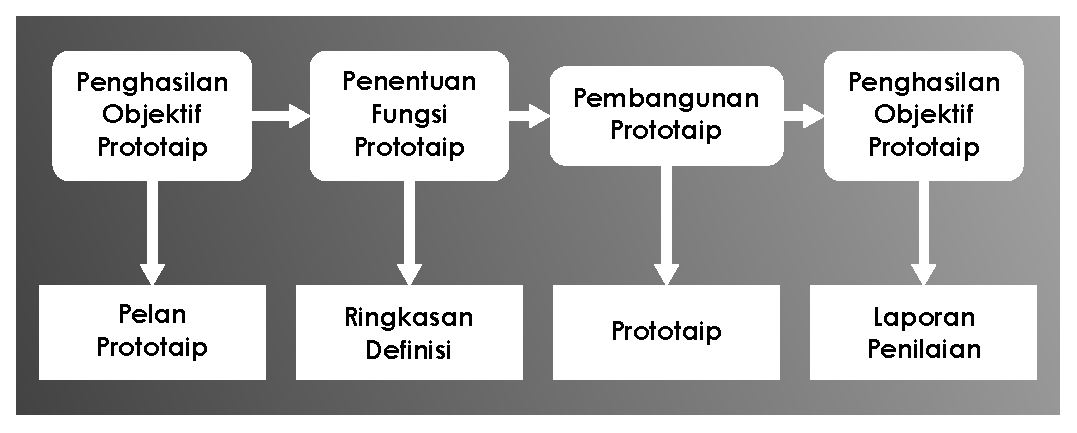
\includegraphics[width=1\textwidth]{source/fig/prototaip.eps}}
\caption[Proses Pembangunan Prototaip]{Proses Pembangunan Prototaip}
\label{c3:f1}
\end{figure}

Dalam pembangunan sistem ini, model prototaip Evolusi digunapakai dalam pembangunan projek. Prototaip Evolusi melaksanakan proses analisis, rekabentuk dan implementasi bersama-sama. Ini bagi memastikan bahawa idea dan teori yang difikirkan dapat dibuktikan setelah prototaip pertama dibina dan diuji pada perkakasan sebenar. Prototaip ELWI yang awalnya dibina di dalam komputer pembangunan dan kemudiannya dipasang kedalam perkakasan terbenam. Fungsi-fungsi baru akan diuji bagi memastikan ia tidak menjejaskan sistem sedia ada. Proses ini diulang berkali-kali sehinggalah sistem siap dibangunkan.

\subsection{Fasa Perancangan}
Peringkat pertama dalam proses pembangunan sistem ialah Fasa Perancangan. Dalam fasa ini, aktiviti yang dilakukan adalah berkaitan kajian awal bagi sistem yang ingin dibangunkan. Antara kajian-kajian yang dilakukan ialah mengenalpasti matlamat, objektif pembangunan sistem, skop-skop dan penyataan masalah berserta kekangan yang dihadapi semasa pembangunan sistem. 

Perancangan kerja untuk membangunkan sistem dilakukan menggunakan Carta Gantt. Penggunaaan Carta Gantt dapat memberikan perkumpulan terhadap tarikh-tarikh penting supaya segala aktiviti-aktiviti pembangunan sistem dapat berjalan seperti yang dirancangkan.

\begin{figure}[!h]
\centering{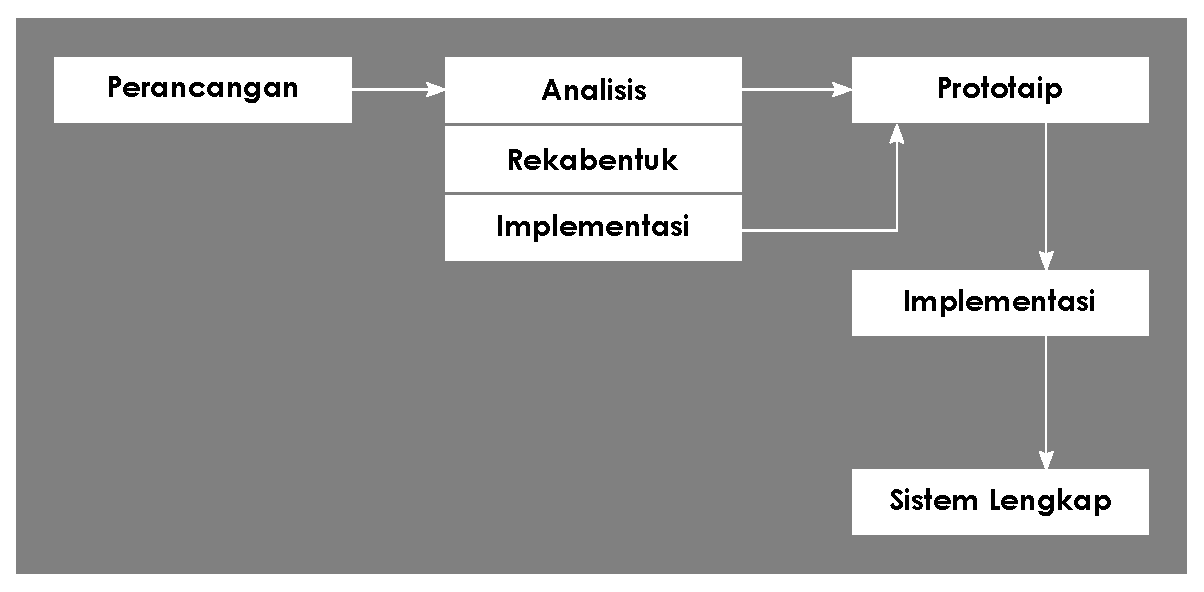
\includegraphics[width=1\textwidth]{source/fig/proto-evolusi.eps}}
\caption[Fasa-fasa Pembangunan Model Prototaip Evolusi]{Fasa-fasa Pembangunan Model Prototaip Evolusi}
\label{c3:f2}
\end{figure}

Tujuan utama fasa ini adalah untuk memberikan pandangan yang jelas serta takrifan awalan bagi sistem yang dibangunkan. Ia adalah penting bagi menjamin kelancaran fasa-fasa yang berikutnya.

\subsection{Fasa Analisis Dan Kajian Awalan}
Kajian awal keatas pembangunan antaramuka pengguna bergrafik untuk mengautomasikan konfigurasi sistem terbenam Linux telah dilakukan bagi mengetahui keperluan dan kemungkinan permasalahan yang akan timbul dalam penghasilan produk akhir kajian ini. Ianya perlu bagi mengenalpasti objektif umum kepada penyelesaian masalah skop serta rancangan selanjutnya. Fasa ini mengenalpasti kenapa sistem baru diperlukan dan matlamat sebenar yang ingin dicapai daripada projek ini.

Bagi projek ini, antaramuka pengguna bergrafik diperlukan untuk mempermudahkan konfigurasi sistem terbenam Linux dan menjadikannya lebih mesra pengguna. Walaupun ini telah dijelaskan dengan lebih lanjut dalam bab yang lalu, dapat disimpulkan bahawa projek ini bertujuan untuk menghasilkan antaramuka pengguna bergrafik bagi sistem terbenam Linux yang menjadikan produk sistem terbenam Linux lebih interaktif dan dapat dikonfigur oleh pengguna akhir tanpa perlu mempunyai asas penggunaan sistem pengoperasian Linux.

Bagi tujuan analisis ialah untuk menganalisa masalah yang telah dikenalpasti sebelum ini dengan lebih terperinci. Analisa masalah ini dilakukan untuk mendapatkan jawapan kenapa perlunya pembangunan ini dan apakah masalah yang perlu diselesaikan oleh hasil pembangunan yang akan dilaksanakan ini. Daripada perbincangan yang telah diterangkan dalam bab-bab yang lepas, masalah sistem sedia ada ialah:
\begin{itemize}
\item Ketiadaan antaramuka yang mesra pengguna dalam sistem terbenam Linux ini.
\item Kesusahan pengguna akhir untuk membuat konfigurasi menggunakan Command Line Interface.
\item Keperluan pra penggunaan (pre-requisite) untuk mempelajari asas sistem pengoperasian Linux untuk nembuat konfigurasi Sistem Terbenam Linux.
\end{itemize}

\subsection{Fasa Rekabentuk}
Tujuan utama fasa ini adalah untuk mentafsir spesifikasi keperluan ke dalam bentuk tersusun yang boleh dilaksanakan pada fasa seterusnya iaitu fasa implementasi. Semasa fasa ini, analisis terperinci dilakukan terhadap proses-proses yang terdapat dalam aplikasi dan setiap interaksi proses dengan data telah dikaji.

Fasa rekabentuk melibatkan kepada keseluruhan sistem meliputi pangkalan data, input, output, keselamatan serta senibina perisian. Komponen-komponen aplikasi dan rekabentuk antaramuka pengguna telah dihasilkan dalam fasa ini. Fasa ini dihuraikan secara mendalam dalam Bab 4.

\subsection{Fasa Implimentasi}
Fasa ini memulakan pembangunan aplikasi secara teknikal dan pembangunan kod aturcara sistem. Pengaturcaraan sistem ini menggunakan text editor Geany dan diuji menggunakan Linux yang dipasang di dalam VMware Player. Linux minimum ini telah dipasang dengan pelayan web Lighttpd, PHP, dan FastCGI untuk menjalankan antaramuka web yang dibangunkan. Oleh kerana sistem ini tidak menggunakan sebarang pangkalan data, maka tiada pangkalan data dipasang kedalam sistem ini.

Fasa implementasi merupakan fasa di mana segala analisis dan kajian rekabentuk ditranformasikan kepada aplikasi boleh guna untuk menyelesaikan masalah. Dalam fasa ini, ELWI dibangunkan menggunakan bahasa pengaturcaraan PHP untuk menjana tag HTML yang membentuk antaramuka bergrafik pada pelayar web pengguna, manakala Bash pula digunakan untuk melakukan fungsi-fungsi konfigurasi dalam sistem terbenam Linux

\subsection{Fasa Pengujian}
Aplikasi yang telah siap dibangunkan diuji bagi memastikan tahap keberkesanannya adalah konsisten semasa ianya digunakan sebagai aplikasi penyelesaian masalah. Aplikasi ini diuji dalam pelbagai peringkat iaitu pengujian fungsi, pengujian integrasi dan pengujian aplikasi. Pengujian-pengujian ini dilakukan sama ada semasa proses pengekodan dan juga pada fasa pengujian bagi memastikan output yang dihasilkan adalah konsisten dan tidak bercanggah dengan objektif yang ingin dicapai.

\section{Keperluan Sistem}
Dalam seksyen Keperluan Sistem ini, kita membincangkan pemilihan perkakasan dan perisian untuk membangunkan antaramuka web yang dipanggil ELWI.

\subsection{Keperluan Perkakasan}

Spesifikasi perkakasan terbenam dipilih berdasarkan keupayaannya untuk melaksanakan tugas khusus sistem terbenam tersebut.

\subsection{Spesifikasi Perisian}

\section{Kesimpulan}
Secara ringkasnya, bab ini menjelaskan setiap perincian kaedah penyelesaian yang diambil meliputi keperluan kepada perisian, perkakasan dan pendekatan metodologi yang digunakan semasa pembangunan aplikasi ini. Tujuan ianya dilakukan adalah sebagai suatu langkah mengenalpasti potensi dan peluang dalam penyelesaian masalah, menggariskan panduan sistematik kepada penyelesaian yang diambil, dan merencanakan rancangan dan fasa-fasa
tindakan selanjutnya bagi melicinkan lagi proses-proses pembangunan dan kajian yang dilakukan.
